
\section{Generating Exchanges}\label{method:setup}

This section focuses on two distinct \textit{species} of exchanges, those
related to the \textit{front end} of the nuclear fuel cycle and those related to
the \textit{back end} of the nuclear fuel cycle. Broadly, the front end of the
fuel cycle is concerned with fueling reactors, and the back end is concerned
with either recycling or disposing of used fuel exiting reactors. Common
features to both types of exchange generation are described in \S
\ref{method:setup:features}.

\S \ref{abm:dre}, however, only describes the methodology for solving a single
exchange. Therefore, an argument must be made for why it is possible to split a
single exchange into multiple exchanges, and specifically why that is valid in
the case of the front and back ends of the NFC. Such an argument is made in \S
\ref{method:setup:split}.

Exchange generation is defined by two types parameters, \textit{exchange} and
\textit{species} parameters. Exchange parameters apply to any species of
exchange, and species parameters apply to a specific species. \S
\ref{method:setup:params} provides a discussion of exchange parameters. \S
\ref{method:setup:front} and \ref{method:setup:back} then follow with a full
description of modeling assumptions and species parameters included for
generating both species of exchanges.

\subsection{Common Features}\label{method:setup:features}

\subsubsection{Fuel Cycles and Commodities}

Three types of fuel cycles can be generated: a once-through fuel cycle (OT), a
plutonium-recycle fuel cycle (MOX), and a plutonium and thorium-recycle fuel
cycle (MOX-ThOX). As fuel cycles increase in complexity, the number of
commodities that exist increases, as shown in Table \ref{tbl:fc_to_commods}. The
commodities are referred to by abbreviation: Enriched Uranium Oxide (UOX), Mixed
Plutonium Oxide for Thermal Reactors (TMOX), Mixed Plutonium Oxide for Fast
Reactors (FMOX), Thorium Oxide for Fast Reactors (FThOX).

\begin{table}[h]
\centering
\caption{A mapping between fuel cycles to their associated commodities.}
\label{tbl:fc_to_commods}
\begin{tabular}{|c|c|}
\hline
Fuel Cycle            & Commodities \\ \hline
OT                    & UOX         \\ \hline
\multirow{3}{*}{MOX}  & UOX         \\  
                      & TMOX        \\  
                      & FMOX        \\ \hline
\multirow{4}{*}{ThOX} & UOX         \\  
                      & TMOX        \\  
                      & FMOX        \\  
                      & FThOX       \\ \hline
\end{tabular}
\end{table}

\subsubsection{Reactors}

All reactors are modeled as either thermal or fast reactors. Thermal reactors
are simplified models of AP-1000 reactors \cite{ARIS}, and fast reactors are
simplified models of BN-600 reactors \cite{reactors2007experience}. Using the
dimensions in Table \ref{tbl:rx_params}, one can estimate that the AP-1000 core
volume is approximately 12.5 times larger than the BN-600 core. 

\begin{table}[h]
\centering
\caption{Primary Reactor Parameters}
\label{tbl:rx_params}
\begin{tabular}{|c|c|c|c|}
\hline
Reactor & Core Height (m) & Core Diameter (m) & Number of Assemblies \\ \hline
AP1000  & 4.27            & 3.04              & 157 \\ \hline
BN600   & 0.75            & 2.05              & 369 \\ \hline
\end{tabular}
\end{table}

Reactors are assumed to to operate in a batch mode, where each batch is
approximately one quarter of the reactor core, similar to other analyses
\cite{rineiski2011reactivity}. Additionaly, a single AP-1000 fuel assembly is
assumed to contain 450 kg of material \cite{kok2009nuclear}. Therefore, a single
batch of thermal reactor fuel is assumed to be

\begin{equation}
   450 \frac{kg}{assembly} * \frac{t}{1000 \: kg} * 157 \frac{assemblies}{core}
   * \frac{1}{4} core = \: \sim 17.6 t.
\end{equation}

The amount of fuel required and number of assemblies by each reactor type is
shown in Table \ref{tbl:rx_batch}. The number of assemblies is taken as the
ratio of total number of assemblies and number of batches per core rounded to
the nearest integer. The batch size for the BN600 reactor is estimated by
dividing the AP1000 batch size by the relative core volume.

\begin{table}[h]
\centering
\caption{Reactor Batch Size}
\label{tbl:rx_batch}
\begin{tabular}{|c|c|c|c|}
\hline
Reactor & Quantity (t) & Number of Assemblies \\ \hline
AP1000  & 17.6          & 39 \\ \hline
BN600   & 1.41          & 92 \\ \hline
\end{tabular}
\end{table}

The reactors that operate in a given exchange is also a function of the fuel
cycle being modeled. In a OT fuel cycle, only thermal reactors exist. In the MOX
case, fast reactors that prefer MOX-based fuel are added and denoted as FMOX
reactors. Finally, in the MOX-ThOX case, an additional class of fast reactor is
added that prefers ThOX-based fuels and is denoted as FThOX. A summary of
available types of reactors as a function of the fuel cycle being modeled is
shown in Table \ref{tbl:fc_to_rxs}. 

\begin{table}[h]
\centering
\caption{A mapping between fuel cycles to the reactor types that exist in exchange instances.}
\label{tbl:fc_to_rxs}
\begin{tabular}{|c|c|}
\hline
Fuel Cycle            & Reactor Types \\ \hline
OT                    & Thermal         \\ \hline
\multirow{3}{*}{MOX}  & Thermal         \\  
                      & FMOX        \\ \hline
\multirow{4}{*}{ThOX} & Thermal         \\  
                      & FMOX        \\  
                      & FThOX       \\ \hline
\end{tabular}
\end{table}

Reactors may be fueled by different commodities. In other words, reactors have a
set of commodities that they either supply or demand, based on the exchange
species being modeled. The set of commodities that reactors can use is a
modeling assumption and a proxy for how reactors may behave in simulations; this
particular reactor-to-commodity mapping may not be true for other analysts' fuel
cycle models. However, it is appropriate to make certain broad assumptions for
such an exploratory study. A mapping of reactors to acceptable commodities is
provided in Table \ref{tbl:rx_to_commods}. Note that there is still a
preference distribution associated with each reactor-commodity pair as well as
constraint coefficient effects. Accordingly, each reactor-commodity pair
provides a unique effect on an exchange instance.

\begin{table}[h]
\centering
\caption{A mapping between reactor types and the commodities allowed to fuel each reactor type.}
\label{tbl:rx_to_commods}
\begin{tabular}{|c|c|}
\hline
Reactor Types            & Fuel Commodities \\ \hline
\multirow{3}{*}{Thermal}                    & EUOX         \\ 
                      & TMOX        \\  
                      & FMOX       \\ \hline
\multirow{4}{*}{FMOX}  & EUOX         \\  
                      & TMOX        \\ 
                      & TMOX        \\  
                      & FThOX        \\ \hline 
\multirow{4}{*}{FThOX} & EUOX         \\  
                     & TMOX        \\ 
                      & TMOX        \\  
                      & FThOX        \\ \hline 
\end{tabular}
\end{table}

\subsubsection{Support Facilities}

In a front-end exchange, fuel suppliers exchange material with reactors. In a
back-end exchange, reprocessing and storage facilities exchange material with
reactors. In either case, facilities that are \text{not} reactors are referred
to as \textit{support} facilities, or \textit{supporters}, as they support the
reactos which generate power. Support facilities for front-end exchanges are
described in \S \ref{method:setup:front:sup}, and support facilities for
back-end exchanges are described in \S \ref{method:setup:back:sup}.

\subsubsection{Preferences}\label{method:setup:features:prefs}

Preferences for all transactions have a default value, $p_{c}(i, j)$, based on
the proposed commodity to be transferred which are defined in species-specific
sections, \S \ref{method:setup:front} and \ref{method:setup:back}. However, a
large exchange with a small preference distribution can lead to problem
degeneracy. Further, a primary application for Cyclus is the modeling of
regional and location effects on fuel cycles. Accordingly, a location proxy is
provided for preferences, as shown in Equation \ref{eqn:loc_proxy}.

Each facility is assigned a location value, $loc_i \in [0, 1)$. The domain is
  then divided evenly into ten regions, where the first region comprises all
  location values in $[0, 0.1)$, and so on. $\delta_{reg}$ and $\delta_{loc}$
    are binary variables which are activated based on the parameters described
    in \S \ref{method:setup:params}. The exponential of the negative absolute
    difference between two regions or locations was chosen as the preference
    function in order to model having higher preferences for closer entities.

\begin{equation}\label{eqn:loc_proxy}
p_{l}(i, j) = \delta_{reg} \frac{\exp(- | reg_{i} - reg_{j} | ) + \delta_{loc}
  \exp(- \| loc_{i} - loc_{j} \| )}{1 + \delta_{loc}}
\end{equation}

The preference for a given arc is then a weighted combination of location and
commodity preferences as shown in Equation \ref{eqn:total_pref}. The weighting
factor, $r_{l, c}$, is a parameter of exchange generation and described further
in \S \ref{method:setup:params}.

\begin{equation}\label{eqn:total_pref}
p(i, j) = p_{c}(i, j) + r_{l, c} p_{l}(i, j)
\end{equation}

\subsection{Splitting Exchanges}\label{method:setup:split}

A well known simplification of the Multicommodity Transportation Problem occurs
when supply and demand is separate for separate commodities. The large
multicommodity problem can then be decomposed into $n$ single commodity
subproblems, where $n$ is the number of commodities. Each subproblem can be
solved separately from the others.

An analog exists in the NFCTP when the Exchange Graph is \textit{separable}. A
bipartite graph with directed arcs, $A$, consisting of sending nodes, $U$, and
receiving nodes, $V$, is separable if there a partition

\begin{equation}
  A = A_{1} \cup A_{2}
\end{equation}

\begin{equation}
  U = U_{1} \cup U_{2}
\end{equation}

\begin{equation}
  V = V_{1} \cup V_{2}
\end{equation}

such that no node in $U_1$ is connected to a node in $V_2$ and no node in $U_2$
is connected to a node in $V_1$. The graph shown in Figure \ref{fig:basic_part} is an
example of a separable bipartite graph.

\begin{figure}
  \begin{center}
    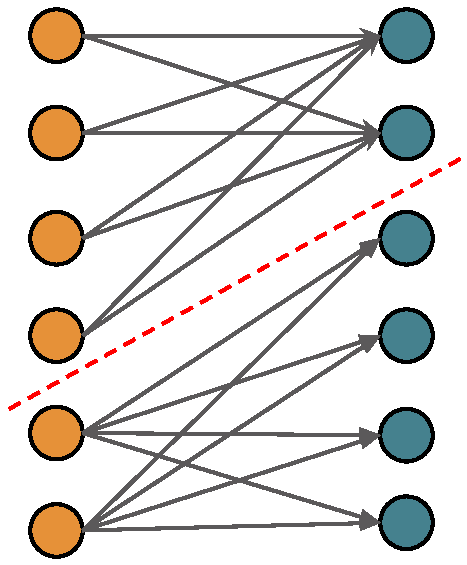
\includegraphics[width=0.55\textwidth]{exchange_part_supreq.pdf}
    \caption[]{
      \label{fig:basic_part}
      A separable bipartite graph with the partition shown as a red 
      dashed line.}
  \end{center}
\end{figure}

The Exchange Graph of the NFCTP, however, has additional structure in the form
of portfolios and thus has a stricter notion of separability. Specifically, the
partition must also separate the set of supplier portfolios, $S$, and requester
portfolios, $R$, as in Equations \ref{eqn:sup_part} and \ref{eqn:req_part},
respectively.

\begin{equation}\label{eqn:sup_part}
  S = S_{1} \cup S_{2}
\end{equation}

\begin{equation}\label{eqn:req_part}
  R = R_{1} \cup R_{2}
\end{equation}

Figure \ref{fig:port_part} depicts a separable Exchange Graph, for example,
while Figure \ref{fig:port_no_part} shows an Exchange Graph that is not
separable, even though the underlying bipartite graph is, due to the lack of a
fully separable portfolio partition.

\begin{figure}
  \begin{center}
    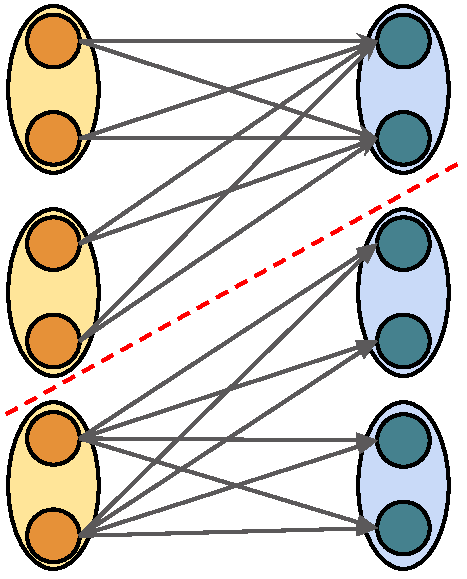
\includegraphics[width=0.55\textwidth]{exchange_part_port.pdf}
    \caption[]{
      \label{fig:port_part}
      A separable Exchange Graph with nodes grouped by portfolio and the
      separating partition shown as a red dashed line.}
  \end{center}
\end{figure}

\begin{figure}
  \begin{center}
    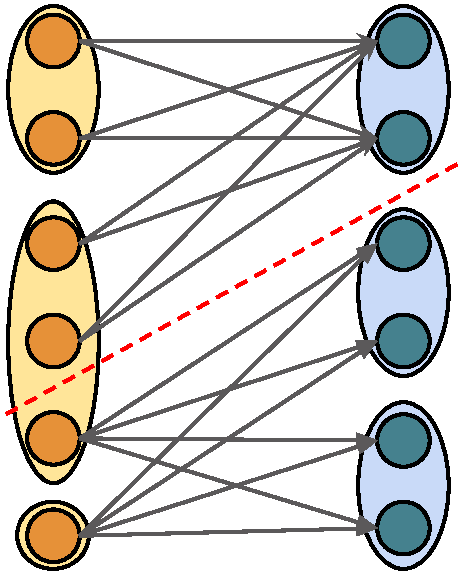
\includegraphics[width=0.55\textwidth]{exchange_no_part_port.pdf}
    \caption[]{
      \label{fig:port_no_part}
      An Exchange Graph with nodes grouped by portfolio that is \textit{not}
      separable because a portfolio crosses the node partition.}
  \end{center}
\end{figure}

The Exchange Graph resulting from the information gathering phase of the DRE
specifically from a NFC application will be minimally separable into front-end
and back-end exchanges if two conditions are met:

\begin{enumerate}
  \item Reactors output commodities can \textit{not} be sent to both other
    reactors and supporting facilities.

  \item Supporting facility output commodities can \textit{not} be sent to both
    other supporting facilities and reactors.
\end{enumerate}

In the first case, separability is broken by a supplier providing bids across a
separating partition. An minimal example is shown in Figure
\ref{fig:no_part_front}. This case can arise if reactors can somehow directly
refuel other reactors. In the NFC domain, such an arrangement only occurs in a
self-recycling system implemented in such a way that a reactor resupplies
itself, which is an abstraction of reality. It is reasonable for a
self-recycling reactor to be implemented in such a way that it does not
participate in the DRE for self-refueling purposes. Accordingly, this condition
is expected to be met in most usage of the DRE.

\begin{figure}
  \begin{center}
    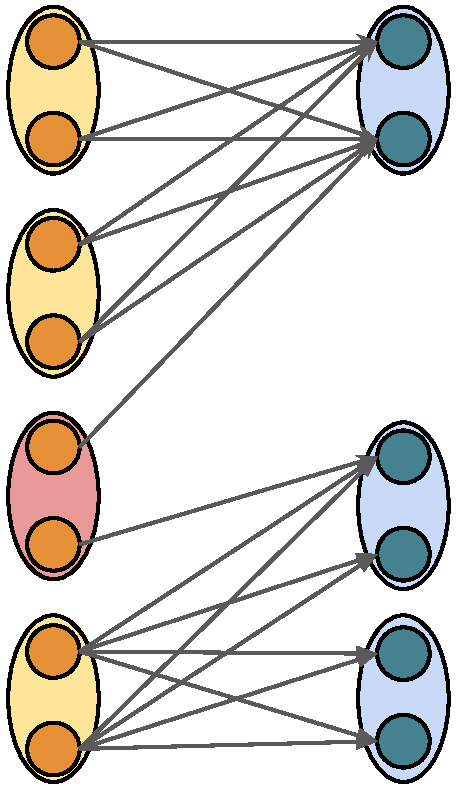
\includegraphics[width=0.55\textwidth]{exchange_no_part_front.pdf}
    \caption[]{
      \label{fig:no_part_front}
      An Exchange Graph separability broken by a supplier. This occurs in NFC
      modeling if assumption $1$ is broken.}
  \end{center}
\end{figure}

In the second case, separability is broken by a requester requesting commodities
across a separating partition. Again, a minimal example is shown in Figure
\ref{fig:no_part_back}. This case can arise in practice when modeling an NFC
system if both a reactor and a repository compete for some commodity. While this
is a valid modeling case under certain assumptions and simplifications, it is
not very realistic. In general fuel that can be used by a reactor has been
processed differently than material to be sent to a repository. Accordingly,
while some analyzed fuel cycles will not meet this requirement, it is assumed
that the vast majority will. If an instance of a DRE does not meet this
requirement, it will not be able to be subdivided into smaller instances.

\begin{figure}
  \begin{center}
    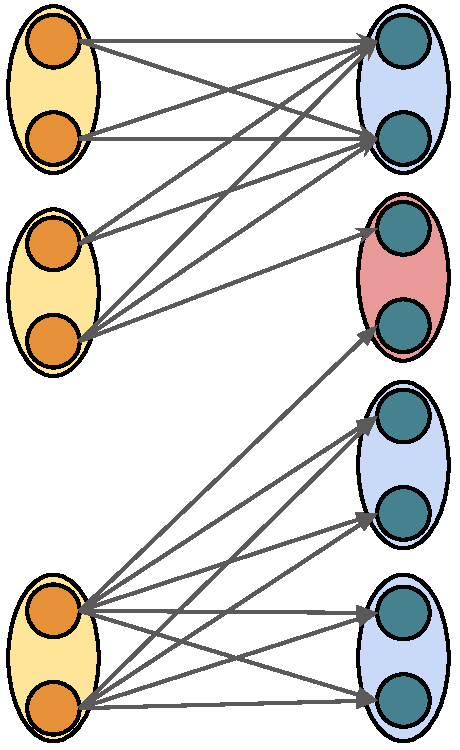
\includegraphics[width=0.55\textwidth]{exchange_no_part_back.pdf}
    \caption[]{
      \label{fig:no_part_back}
      An Exchange Graph separability broken by a requester. This occurs in NFC
      modeling if assumption $2$ is broken.}
  \end{center}
\end{figure}

Because the majority of fuel cycles analyzed will meet both conditions, the
majority of DRE instances will be able to be separated into two distinct
instances which can solved independently of one another. One instance will be
associated with the front end of the fuel cycle where reactors are requesting
fuel. The other instance will be associated with the back end of the fuel cycle,
where reactors are supplying used fuel.

\subsection{Exchange Parameters}\label{method:setup:params}

The generation of exchanges is naturally a parameterized process. For instance,
a critical parameter is the number of reactors in an exchange. Exchange
generation parameters can be divided into two classifications, fundamental
parameters and instance parameters. All exchange species share some fundmental
parameters and instance parameters. Species also define their own set of
instance parameters to complete the full set of parameters needed to define and
instance of an exchange.

\subsubsection{Fundamental Parameters}

The fundamental parameters are related to the common features of all species
described in \S \ref{method:setup:features}. Each parameter is a switch that
sets the level of fidelity of a given exchange. As such, they are each denoted
as $f_x$, where the $x$ subscript describes the parameter.

The most critical parameter is related to the fidelity of the fuel cycle being
modeled, $f_{fc}$. A value of zero indicates modeling the OT fuel cycle, one is
used for the MOX fuel cycle, and two the ThOX fuel cycle. As fuel cycle fidelity
increases, the number of commodities increases, and thus the number of possible
connections between suppliers and consumers that exist increases as some
entities trade in multiple commodities. The fuel cycle parameter has an integer
mapping to the modeled fuel cycle for conveniance as shown in Table
\ref{tbl:ffc}.

\begin{table}[h]
\centering
\caption{A mapping between fuel cycles and $f_{rx}$ values.}
\label{tbl:ffc}
\begin{tabular}{|c|c|}
\hline
Fidelity (Fuel Cycle)            & $f_{fc}$ \\ \hline
UOX                    & 0         \\ \hline
MOX                    & 1         \\ \hline
ThOX                    & 2         \\ \hline
\end{tabular}
\end{table}

The second parameter is reactor fidelity, $f_{rx}$. Reactors can either make
requests or provide supply based either on their entire batch or for each
assembly in a batch. A value of zero indicates reactors trading full batches; a
value of one indicates reactors trading individual assemblies. Trading
individual assemblies is of higher fidelity because the number of trades
increases by nearly an order of magnitude. Again, there is a mapping between the
meaning of the reactor fidelity parameter and integer values as shown in Table
\ref{tbl:frx}.

\begin{table}[h]
\centering
\caption{A mapping between reactor fidelity and $f_{rx}$ values.}
\label{tbl:frx}
\begin{tabular}{|c|c|}
\hline
Fidelity            & $f_{rx}$ \\ \hline
Batches                    & 0         \\ \hline
Assemblies                    & 1         \\ \hline
\end{tabular}
\end{table}

Finally, the fidelity with with objective value coefficients are generated can
be varied. This parameter is denoted $f_{loc}$ because it is related to the
degree to which location is taken into account in Equation
\ref{eqn:loc_proxy}. The mapping between $f_{loc}$ and parameters in Equation
\ref{eqn:loc_proxy} is shown in Table \ref{tbl:floc}. As $f_{loc}$ increases,
the size of the distribution of possible objective coefficent values increases.

\begin{table}[h]
\centering
\caption{$f_{loc}$ Effects on Objective Coefficient Values}
\label{tbl:floc}
\begin{tabular}{|c|c|c|c|}
\hline
Fidelity & $f_{loc}$ &$\delta_{reg}$ & $\delta_{loc}$ \\ \hline
No location data & 0  & 0          & 0 \\ \hline
Region location data & 1   & 1          & 0 \\ \hline
Region and actual location data & 2   & 1          & 0 \\ \hline
\end{tabular}
\end{table}

\subsubsection{Instance Parameters}

While fundamental parameters represent switches that change the notion of the
exchange being generated, for example the difference between a once-through fuel
cycle and a fuel cycle with recycling, instance parameters change the
\textit{shape} and \textit{size} of instances in a given population. Given an
instance's shape and size, instance parameters can also affect
\textit{coefficient generation}. In other words, fundamental parameters are
related basic modeling assumptions while instance parameters are related to the
specifics of an instance, given those basic modeling assumptions. Both speices
of exchange instances share some instance parameters, namely those related to
the population of reactors in a given exchange and coefficient generation
parameters related to objective coefficients.

\paragraph{Reactor Population}

Instances are broadly defined by a parameter representing the number of reactors
that exist in an exchange instance, $n_{rx}$. Next, the split between thermal
and fast reactors is defined by a ratio, $r_{th, f}$. Assuming $f_{fc} > 0$, the
number of thermal and fast reactors is given by

\begin{equation}
n_{rx, th} = r_{th, f} * n_{rx},
\end{equation}

and 

\begin{equation}
n_{rx, f} = n_{rx} - n_{rx, th},
\end{equation}

otherwise, a OT fuel cycle is modeled, thus $n_{rx}$ is equal to $n_{rx, th}$ as
there are only thermal reactors in the exchange. If a MOX fuel cycle is modeled,
the number of FMOX reactors, $n_{rx, fmox}$ is trivially equal to the number of
fast reactors. However, for a ThOX fuel cycle, i.e., $f_{fc} > 1$, the number of
FMOX and FThOX reactors is determined by a ratio parameter $r_{rx, fthox, fmox}$
such that 

\begin{equation}
n_{rx, fthox} = r_{rx, fthox, fmox} * n_{rx, f}
\end{equation}

and

\begin{equation}
n_{rx, fmox} = n_{rx, f} - n_{rx, fthox}.
\end{equation}

In the event that the determined number of reactors is non integral, the value
is rounded to the nearest integer, with an imposed minimum value of unity.

\paragraph{Objective Coefficients}

As shown in Equation \ref{eqn:total_pref}, the value of an objective coefficient
has two components, preference due to a commodity transfer, $p_c$, and
preference due to the relative location between two entities, $p_l$. It is not
obvious to what degree, if any, the relative values of the two components affect
formulation performance. Accordingly, a ratio parameter, $r_{l, c}$ is
introduced to allow for investigating such effects.

\subsubsection{Parameter Summary}

A summary of species-independent parameters is provided in Table
\ref{tbl:global_params}.

\begin{table}[h]
\centering
\caption{Parameter Description Summary for Species-Independent Parameters.}
\label{tbl:global_params}
\begin{tabularx}{\columnwidth-10pt}{|c|c|X|} % line wraps second column if too long
\hline
Parameter    & Type &
Description
\\ \hline
$f_{fc}$     & Fundamental &
The fuel cycle fidelity of an instance (which fuel cycle is being modeled).
\\ \hline
$f_{rx}$   & Fundamental &
The reactor fidelity of an instance (whether individual assemblies are modeled
or whole batches are modeled).  
\\ \hline
$f_{loc}$    & Fundamental &
The location fidelity of an instance (to what degree is facility location
included in objective coefficients).
\\ \hline
$n_{rx}$   & Instance &
The number of reactors in an instance.
\\ \hline
$r_{rx, t, f}$   & Instance &
The ratio of thermal to fast reactors in an instance, if appropriate.
\\ \hline
$r_{rx, th, pu}$ & Instance &
The ratio of ThOX-based fast reactors to MOX-based fast reactors, if appropriate.
\\ \hline
$r_{rx, th, pu}$ & Instance &
The ratio of ThOX-based fast reactors to MOX-based fast reactors, if appropriate.
\\ \hline
$r_{l, c}$ & Instance &
The weight given to location preference with respect to commodity preference.
\\ \hline
\end{tabularx}
\end{table}

\subsection{Front-End Exchanges}\label{method:setup:front}

A front-end exchange is one in which reactors request fuel and supporting
facilities supply fuel material. \S \ref{method:setup:front:sup} describes how
the population of supporting facilities is determined. Conceptually, the
information gathering procedure for this exchange begins with the RFB phase
where reactors make requests for commodities with a given quantity and
enrichment. Enrichment in this case is a simple proxy for an isotopic
vector. Supporting facilities are then polled to provide a response to these
requests during the RRFB phase. Managers of reactors would then adjust
preferences based on implemented strategies. The remainder of this section
describes how front-end exchange generation models the information gathering
procedure, starting with the generation of requests in \S
\ref{method:setup:front:reqgen}, followed by the generation of supply responses
in \S \ref{method:setup:front:subgen}. The PA phase is modeled using the
location proxy described in \S \ref{method:setup:features:prefs}. Throughout the
discussion on generating front-end exchanges, instance parameters are defined. A
summary of all front-end specific instance parameters is described in \S
\ref{method:setup:front:sum}.

\subsubsection{Support Facility Population} \label{method:setup:front:sup}

It is assumed that there is a single type of supporter for each type of commodity
used in the fuel cycle described in Table \ref{tbl:fc_to_commods}. Therefore
there are four types of supporters, directly mapping to commodities as shown in
Table \ref{tbl:commod_to_sup}.

\begin{table}[h]
\centering
\caption{A mapping between commodities and the supporter type of that commodity.}
\label{tbl:commod_to_sup}
\begin{tabular}{|c|c|}
\hline
Commodities            & Supporter \\ \hline
UOX                    & UOX         \\ \hline
TMOX                    & TMOX         \\ \hline
FMOX                    & FMOX         \\ \hline
FThOX                    & FThOX         \\ \hline
\end{tabular}
\end{table}

The number of each type of supporter in a front-end exchange instance is a
function of of the number of type of reactor as well as configurable
parameters. Supporter types are divided into two groups: those who primarily
support thermal reactors and those who primarily support fast reactors. The
number of thermal fuel supporters is determined to be the product of the number
of thermal reactors and a ratio parameter, $r_{s, th}$, such that the number of
thermal supporters is

\begin{equation}
n_{s, th} = r_{s, th} * n_{rx, th}.
\end{equation}

The number of TMOX supporters, assuming $f_{fc} > 0$ is then determined by a
similar ratio parameter, $r_{s, tmox, uox}$, such that the number of UOX and
TMOX supporters is

\begin{equation}
n_{s, tmox} = r_{s, tmox, uox} * n_{s, th}
\end{equation}

and

\begin{equation}
n_{s, uox} = n_{s, th} - n_{s, tmox}.
\end{equation}

The number of fast reactor fuel supporters is determined directly from the number
of associated fast reactors in the exchange using similar ratio parameters,
$r_{s, fmox}$ and $r_{s, fthox}$. Assuming $f_{fc} > 0$, the number of FMOX
supporters is given as

\begin{equation}
n_{s, fmox} = r_{s, fmox} * n_{rx, fmox}.
\end{equation}

Similarly, assuming $f_{fc} > 1$, the number of FThOX supporters is given as  

\begin{equation}
n_{s, fthox} = r_{s, fthox} * n_{rx, fthox}.
\end{equation}

\subsubsection{Request Generation}\label{method:setup:front:reqgen}

Reactors make \textit{mutual} requests for all commodities that they can consume
as described in Table \ref{tbl:rx_req}. In batch mode, i.e., when $f_{rx}$
equals zero, a single request is made per commodity. In assmebly mode, a request
is made per assembly per commodity, with the number of assemblies denoted
previously in Table \ref{tbl:rx_params}. A single request portfolio encompasses
all requests, with a portfolio quantity equal to the reactor's batch size.

It is assumed that fuel is requested at some enrichment level dependent on the
reactor type. Each reactor in an exchange will choose a batch enrichment level
given a uniform distribution. Further, it is assumed that all recycled fuel is
composed of a target element oxide and topped up with natural uranium oxide. The
mixing ratios is again based on reactor type. For recycled fuel, the associated
enrichment level describes the enrichment of the fissile isotope in the
\textit{target} element. For example, MOX fuel with 45\% enrichment implies that
of the elemental Plutonium in the mixture, 45\% is comprised of isotopic
\nucl{239}{Pu}. Finally, each reactor has a preference assignment over its set
of consumable commodities.

Thermal reactors can consume UOX fuel as well as both MOX variants. It is
assumed that thermal reactors would prefer to consume thermal MOX fuel in order
to maintain any equilibrium status of the cycle. UOX fuel is next perferred, and
finally fast MOX, a fuel type usable by but not meant for thermal reactors. A
preference distribution is assumed to be ${1, 0.5, 0.1}$, respectively. A normal
operating enrichment range of $[3.5, 5.5]$ is used for UOX fuel. MOX-based fuels
are assumed to be comprised of 7\% Plutonium with 93\% Uranium top up
\cite{bertel2007management} with an enrichment range of $[55, 65]$
\cite{bairiot2003status}. In practice, many reactor concepts restrict the
fraction of an LWR's core that can be made up of MOX fuel rather than UOX fuel
due to a reduced safety margin. Accordingly, a tuneable parameter is added to
the model, $f_{mox}$, which denotes the fraction of a request that can be made
up of MOX-based fuel. This fraction is only relevant if reactors are operating
in assembly mode, i.e., if $f_{rx}$ is unity.

MOX and ThOX fast reactors utilize the same governing request parameters but
have a different preference distribution over commodities. It is assumed that a
Thorium-based fast reactor prefers Thorium-based fast reactor fuel over
MOX-based fast reactor fuel. Finally, such a reactor can utilize thermal MOX
fuel or medium-enriched UOX, but prefers fast reactor-based fuels. Accordingly,
a preference distribution of ${1, 0.5, 0.25, 0.1}$ is assigned to each
commodity, respectively. A MOX-based fast reactor is assumed to operate
differently, preferring fast and thermal MOX fuel over ThOX fuel. Medium
enriched UOX is again a viable fuel commodity but least preferred. The same
preference value distribution is used. For both fast reactors, a UOX enrichment
range of $[15, 20]$ is used, having an upper limit set by LEU legal enrichment
limits. All recycled fuels commodities are assigned an enrichment range of $[55,
  65]$ \cite{bairiot2003status} and using a composition of 20\% of the target
element (Plutonium or Thorium) and 80\% Uranium top up \cite{bairiot2003status}.

A summary of chosen chosen request parameters based on reactor and commodity
types is shown in Table \ref{tbl:rx_req}.

\begin{table}[h]
\centering
\caption{A summary of reactor request parameters.}
\label{tbl:rx_req}
\begin{tabularx}{\columnwidth-10pt}{@{} *5{|>{\centering\arraybackslash}X}| @{}}
% line wraps second column if too long
\hline
Reactor Type             & Commodity & Enrichment Range & 
Target Element Fraction (\%), $f_{el}$ & Commodity Preference, $p_c$
\\ \hline
\multirow{3}{*}{Thermal} & 
UOX   & $[3.5, 5.5]$         & 100 & 0.5        \\ \cline{2-5} 
& 
TMOX  & $[55, 65]$         & 7 & 1      \\ \cline{2-5} 
& 
FMOX  & $[55, 65]$         & 7 & 0.1      \\ \hline
\multirow{4}{*}{FMOX}    & 
UOX & $[15, 20]$         & 100  & 0.1     \\ \cline{2-5} 
& 
TMOX & $[55, 65]$         & 20 & 0.5      \\ \cline{2-5} 
& 
FMOX & $[55, 65]$         & 20 & 1      \\ \cline{2-5} 
& 
FThOX & $[55, 65]$         & 20 & 0.25      \\ \hline
\multirow{4}{*}{FThOX}   & 
UOX & $[15, 20]$         & 100 & 0.1      \\ \cline{2-5} 
& 
TMOX & $[55, 65]$         & 20 & 0.25      \\ \cline{2-5} 
& 
FMOX & $[55, 65]$         & 20 & 0.5      \\ \cline{2-5} 
& 
FThOX & $[55, 65]$         & 20 & 1      \\ \hline
\end{tabularx}
\end{table}

\subsubsection{Supply Generation}\label{method:setup:front:subgen}

With all requests known, each supporting supply facility responds to all
requests for their assigned commodity, creating an associated supply node and an
arc between the supply node and request node. Constraint coefficients are
supplied for each arc based on the requested enrichment associated with that
arc. Furthermore, a right-hand side (RHS), $\beta^k_s$, is provided for each
constraint in addition to a coefficient conversion function.

Each supplier has two types of constraints for which coefficients must be
calculated: a \textit{process} constraint and an \textit{inventory} constraint. A
process constraint models a situation in which the amount of supplied fuel is
constrained physically; only so much fuel can be made in one time step. An
inventory constraint models a situation in which a supplier is constrained by
the available material inventory on hand. Both constraints are a function of
requested quantity and fuel enrichment.

\paragraph{UOX Constraints}

A UOX supplying facility is assumed to be constrained by a SWU process
constraint and a natural Uranium inventory constraint. Assuming general
operating parameters, including a tails assay of $0.3$ and a feed assay of
natural Uranium, $0.711$, constraint coefficents can be applied to arcs. The SWU
coefficient conversion function is previously described in Equation
\ref{eqs:enr-swu-beta} while the natural Uranium conversion function is
described in Equation \ref{eqs:enr-prod-beta}. Therefore, for UOX supplying
facilities,

\begin{equation}
\beta^{\text{proc}}_s(\epsilon) = \beta^{\text{SWU}}_s(\epsilon) 
\end{equation}

and

\begin{equation}
\beta^{\text{inv}}_s(\epsilon) = \beta^{\text{NU}}_s(\epsilon). 
\end{equation}

In order to determine a constraining RHS, the proposed Eagle Rock Enrichment
Plant is chosen as a model. It purports to have a possible yearly SWU capacity
of $3.3E6$ Million SWU per year. Accordingly, the process constraint RHS is
chosen to be the appropriate monthly value,

\begin{equation}
b^{\text{SWU}}_s = \sim 2.75E5 \frac{\text{SWU}}{\text{month}}.
\end{equation}

An inventory constraint will be based on the present state of a facility and at
given time step in the simulation. Therefore, a sufficiently reasonable value
must be provided without actual simulation data. Accordingly, the process RHS is
multiplied by a translation constant to achieve an equivalent value for an
inventory constraint. The translation constant is taken to be a ratio of
constraint coefficients for the average enrichment of a primary requester. Thus,
a UOX supplying facility uses a average enrichment, $\bar{\epsilon}$, of $4.5$
because that is the median of the thermal reactor enrichment range. Further, a
ratio coefficient parameter, $r_{inv, proc}$, is added in order to investigate
interesting cases from a formulation point of view. If $r_{inv, proc} > 1$, then
the process constraint RHS is smaller and thus the process constraint is more
likely to be engaged in an feasible solution than the inventory constraint. On
the other hand, if $r_{inv, proc} < 1$, the inventory constraint is more likely
to be engaged. Including all of the above conversation, the inventory constraint RHS is chosen to be,

\begin{equation}
b^{\text{inv}}_s = 
r_{inv, proc} 
\frac{\beta^{\text{inv}}_s(\bar{\epsilon})}{\beta^{\text{proc}}_s(\bar{\epsilon})} 
b^{\text{proc}}_s.
\end{equation}

The determination of the inventory RHS is identical for all supporting
facilities.

\paragraph{Recycled Commodity Constraints}

Due to the lack of commercially viable, well documented fast reactor fuel
suppliers, a simple linear surrogate model is assumed for an inventory
constraint. Thus, the coefficient function conversion function is simply 

\begin{equation}
\beta^{\text{inv}}_s(\epsilon) = f_{el} \epsilon. 
\end{equation}

There are many possible process surrogate models that could be used, such as
heat production or radiotoxicity; however, each of these requires a detailed
isotopic composition to be relevant. Per the current IAEA practice
\cite{heinonen2010}, and extrapolating the same effect for reprocessing
\nucl{233}{U}, a factor of 100 is added for for Plutonium and Thorium-based
commodities.

The process constraint coefficient function is then as the mass-based processing
factor

\begin{equation}
\beta^{\text{proc}}_s = 100 f_{el}. 
\end{equation}

From previous conversations with industry representatives \cite{murraycomm}, a
reasonable size for a processing plant is 800 tonnes per year, which is similar
to the Rokkassho plant in Japan \cite{heinonen2010}. With $f_{\text{commod}}$
equal to 100 as discussed above, an 800 t Uranium / 8 t Plutonium facility could
service on the order of 2-3 fast reactors or $\sim$2 thermal reactors with
$\frac{1}{3}$ a request as MOX. The yearly process limit is again translated to
a monthly limit, resulting in a constraint RHS value of

\begin{equation}
b^{\text{proc}}_s = \sim 66.7 \frac{\text{t}}{\text{month}}.
\end{equation}

The inventory constraint RHS is determined identically to the UOX case.

\subsubsection{Parameter Summary}\label{method:setup:front:sum}

A summary of front-end exchange species-depedent instance parameters is provided
in Table \ref{tbl:front_params}.

\begin{table}[h]
\centering
\caption{Parameter Description Summary for Front-End Exchange Instance Parameters.}
\label{tbl:front_params}
\begin{tabularx}{\columnwidth-10pt}{|c|X|} % line wraps second column if too long
\hline
Parameter    & 
Description
\\ \hline
$f_{mox}$     & 
The fraction of thermal reactor requests that can be met with mox fuel.
\\ \hline
$r_{s, th}$ & 
The ratio of thermal support facilities to thermal reactors.  
\\ \hline
$r_{s, tmox, uox}$ & 
The ratio of TMOX to UOX support facilities.
\\ \hline
$r_{s, fmox}$ & 
The ratio of FMOX support facilities to FMOX reators.
\\ \hline
$r_{s, fthox}$ & 
The ratio of FThOX support facilities to FThOX reators.
\\ \hline
$r_{inv, proc}$   & 
The ratio of the inventory RHS to the process RHS.
or whole batches are modeled).  
\\ \hline
\end{tabularx}
\end{table}

\subsection{Back-End Exchanges}\label{method:setup:back}

A back-end exchange models the transfer of used fuel from reactors to supporting
facilities, such as reprocessing facilities and repositories. During the
information gathering process, supporting facilities make requests for
commodities that can either be used directly in the recycling process or need to
be stored, temporarily or permanently. Reactors then respond based on output
fuel to each request during the RRFB phase. Throughout the discussion on
generating back-end exchanges, instance parameters are defined. A summary of all
back-end specific instance parameters is shown in Table \ref{tbl:back_params}.

\subsubsection{Support Facility Population}\label{method:setup:back:sup}

Four classes of supporting facilities are modeled in back-end exchanges: thermal
fuel recycling facilities, a facility that recycles fast MOX fuel, a facility
that recycles fast ThOX fuel, and a repository. As thermal fuel recycling
facilities are the only thermal supporting facilities, the number of such
facilities in a given back-end exchange is trivially $n_{s, th}$. As is the case
with front-end exchanges, there is a class of supporting facility for each fast
fuel commodity. Accordingly, the population of each facility type is identical:

\begin{equation}
n_{s, fmox} = r_{s, fmox} * n_{rx, fmox}
\end{equation}

and

\begin{equation}
n_{s, fthox} = r_{s, fthox} * n_{rx, fthox}.
\end{equation}

Back-end exchanges include repositories, a facility type not present in
front-end exchanges. A simple ratio parameter, $r_{\text{repo}}$ is applied
based on the total number of other supporting facilities, i.e.,

\begin{equation}
n_{s, \text{repo}} = r_{s, \text{repo}} ( n_{s, th} + n_{s, fmox} +n_{s, fthox} ).
\end{equation}

\subsubsection{Request Generation}

It is assumed that any recycling facility will accept UOX fuel. However, MOX
recycling facilities can not process ThOX-based fuels, and ThOX facilities can
not process MOX-based fuels. Additionally, fast MOX facilities prefer fast MOX
fuel, while thermal facilities prefer thermal MOX fuel. Finally, repositories
can accept all commodities; however, it is a consumer of last resort. The
assigned preference distribution as a function of commodity type and supporting
facility type is shown in Table \ref{tbl:sup_to_pref}.

\begin{table}[h]
\centering
\caption{Preference Mapping between Back-End Supporting Facilities and Commodities.}
\label{tbl:sup_to_pref}
\begin{tabular}{|c|c|c|c|c|}
\hline
\backslashbox{Supporting Facility}{Commodity} & UOX & TMOX & FMOX & FThOX \\ \hline
TMOX                & 1     & 1      & 0.5    & N/A     \\ \hline
FMOX                & 0.5   & 1      & 1      & N/A     \\ \hline
FThOX               & 0.3   & N/A    & N/A    & 1       \\ \hline
Repo                & 0.1   & 0.1    & 0.1    & 0.1     \\ \hline
\end{tabular}
\end{table}

A single request for the facility's processing capacity is made for each
commodity. Recycling facilities define their request quantity using the same 800
ton per year limit discussed in \S \ref{method:setup:front}. Repostories,
however, use a limit based on the Yucca Mountain statutory limit of 17,000 tons
and assuming a 30-year operating lifetime, i.e., period of time in which fuel
can enter the facility. Thus, a repostiory's request quantity is determined to
be $\sim 48 \frac{\text{t}}{\text{month}}$.

A fissile quantity constraint is added for each recycling facility. A fissile
constraint is \textit{not} added for reprocessing facilities. The fissile
constraint is used to model a situation in which recycling facilities have a
demand for fissile material. The amount of fissile material required by
recycling facilities is based on their primary consumer. It is determined to be
the product of the facility's mass constraint and the mean amount of fissile
material in a primary consumer's request per unit mass, as shown in Equation
\ref{eqn:bfiss}. This constraint can be translated as ``recycling facilities
request fissile material quantities as if its capacity was completely met by
average primary reactors''.

\begin{equation}\label{eqn:bfiss}
b^{\text{fiss}}_r = \bar{\epsilon} f_{el} b^{\text{mass}}_r.
\end{equation}

The fissile constraint coefficient is simply the amount of fissile material for
a given supply, as described in Equation \ref{eqn:betafiss}.

\begin{equation}\label{eqn:betafiss}
\beta^{\text{fiss}}_r(\epsilon) = \epsilon f_{el}.
\end{equation}

\subsubsection{Supply Generation}

A key difference between the front-end and back-end exchanges is that in
front-end exchanges, reactors request fuel, and thus can make a single request
per commodity per assembly modeled. In back-end exchanges, the commodity
assigned to each assembly must be assigned. Accordingly, a key parameter in
back-end exchanges is the commodity distribution for assemblies. A normalized
uniform distribution parameter exists for each reactor type with a value for
each commodity type that reactor can consume as defined in Equation
\ref{eqn:assemdist}.

\begin{equation}\label{eqn:assemdist}
\begin{split}
d_{\text{Th}} = & \:
[x_{\text{UOX}}, x_{\text{TMOX}}, x_{\text{FMOX}}], \: x_i \in [0, 1) \\
d_{\text{FMOX}} = & \:
[x_{\text{UOX}}, x_{\text{TMOX}}, x_{\text{FMOX}}, x_{\text{FThOX}}], \: x_i \in [0, 1) \\
d_{\text{FThOX}} = & \:
[x_{\text{UOX}}, x_{\text{TMOX}}, x_{\text{FMOX}}, x_{\text{FThOX}}], \: x_i \in [0, 1) 
\end{split}
\end{equation}

If an exchange is in batch mode, i.e., $f_{rx}$ is zero, then this distrbution
acts as a selection distribution, where each $x_i$ represents a probability that
the batch will be of that commodity. If in assembly mode, then commodities are
assigned to each assembly given the relative $x_i$ values.  The assignment of
commodities to number of assemblies for a given reactor type is done by rounding
the product of $x_i$ and the total number of assemblies, starting with the
lowest value of $x_i$. The final assignment is then taken as the difference
between the total number of assmblies and the previously assigne values.

For example, consider a thermal reactor with a distribution $d_{\text{Th}} =
[\frac{2}{3}, \frac{1}{3}, 0]$ and number of assemblies $n_a = 39$. The
following assembly breakdown would be calulated as

\begin{gather*}
n_{\text{FMOX}} = \text{round}(x_{\text{FMOX}} n_a) = 0 \\
n_{\text{TMOX}} = \text{round}(x_{\text{TMOX}} n_a) = 0 \\
n_{\text{UOX}} = n_a - n_{\text{TMOX}} - n_{\text{FMOX}} = 26.
\end{gather*}

Once a commodity is assigned either to a single batch or a selection of
assemblies, the remaining methodology is identical. Accordingly, the following
discussion uses the term assembly to mean either an individual assembly or a
batch. That is, a reactor in a back-end exchange with $f_{rx}$ equal to zero has
a single assembly to supply. If $f_{rx}$ is one, then it has $n_a$ assemblies to
supply.

In order to assign enrichment values to each assembly, a single random value is
chosen, $x \in [0, 1)$. Each assembly is then assigned an enrichment based on
  the assembly's commodity and enrichment range, as defined in Table
  \ref{tbl:rx_req}. This modeling assumption supports a situation in which, for
  a given batch, equivalent fissile enrichments were used across commodities.

A bid portfolio is assigned to each assembly. Given the commodity of each
assembly, a supply response is provided to each supporting facility that requsts
that commodity. For example, given a UOX assembly, a reply is sent to each
supporting facility, as all supporting facilities accept UOX, shown in Table
\ref{tbl:sup_to_pref}. The set of supply responses associated with a single
assembly is denoted a \textit{mutual} set. That is, each supply node corresponds
to a single assembly that should not be split amongst supporting facilites.

\subsubsection{Parameter Summary}

A summary of back-end exchange species-depedent instance parameters is provided
in Table \ref{tbl:back_params}.

\begin{table}[h]
\centering
\caption{Parameter Description Summary for Back-End Exchange Instance
  Parameters.}
\label{tbl:back_params}
\begin{tabular}{|c|c|}
\hline
Parameter    & 
Description
\\ \hline
$d_{\text{Th}}$     & 
thermal reactor assembly distribution
\\ \hline
$d_{\text{FMOX}}$     & 
fast mox reactor assembly distribution
\\ \hline
$d_{\text{FThOX}}$     & 
fast thox reactor assembly distribution
\\ \hline
$r_{\text{repo}}$     & 
repository to supporting facility ratio
\\ \hline
\end{tabular}
\end{table}
